\documentclass[11pt]{article}
\usepackage[a4paper,margin=1in]{geometry}
\usepackage{amsmath,amssymb,amsfonts}
\usepackage{booktabs}
\usepackage{graphicx}
\usepackage{caption}
\usepackage{enumitem}
\usepackage{pgfplots}
\usepackage{pgfplotstable}
\usepackage{tikz}
\usepackage[hidelinks]{hyperref}
\usepackage{microtype}
\setlength{\emergencystretch}{4em}

\usetikzlibrary{calc,arrows.meta}
\pgfplotsset{compat=1.18}
\definecolor{accentA}{RGB}{31,119,180}
\definecolor{accentB}{RGB}{255,127,14}
\definecolor{accentC}{RGB}{44,160,44}
\definecolor{accentD}{RGB}{148,103,189}
\definecolor{accentE}{RGB}{214,39,40}
\pgfplotscreateplotcyclelist{accentcolors}{
{accentA, thick},
{accentB, thick},
{accentC, thick},
{accentD, thick},
{accentE, thick}
}
\pgfplotsset{
  fptaxis/.style={
    width=\linewidth,
    height=4.8cm,
    scale only axis,
    xlabel={$t$},
    ylabel={$f(t)$},
    grid=both,
    major grid style={line width=0.35pt, draw=gray!25},
    minor grid style={line width=0.2pt, draw=gray!15},
    axis line style={black!60},
    tick align=outside,
    tick style={black!60},
    label style={font=\small},
    ticklabel style={font=\footnotesize},
    legend style={font=\scriptsize, draw=none, fill=none},
    cycle list name=accentcolors,
    unbounded coords=jump,
  },
  fptaxislin/.style={
    width=0.78\linewidth,
    height=4.6cm,
    scale only axis,
    xlabel={$t$},
    ylabel={$f(t)$},
    grid=major,
    major grid style={line width=0.35pt, draw=gray!20},
    axis background/.style={fill=gray!3},
    axis line style={black!60},
    tick align=outside,
    tick style={black!60},
    label style={font=\small},
    ticklabel style={font=\footnotesize},
    title style={font=\small},
    legend style={font=\scriptsize, draw=none, fill=none},
    cycle list name=accentcolors,
    unbounded coords=jump,
    line cap=round,
    line join=round,
  },
  scanaxis/.style={
    width=\linewidth,
    height=4.8cm,
    scale only axis,
    view={0}{90},
    colormap={bimodal}{rgb=(0.95,0.95,0.95) rgb=(0.50,0.80,0.72) rgb=(0.98,0.70,0.48)},
    point meta min=0,
    point meta max=2,
    axis line style={black!60},
    tick align=outside,
    tick style={black!60},
    label style={font=\small},
    ticklabel style={font=\footnotesize},
  },
}

\newcommand{\configcard}[1]{%
  \vspace{-6pt}%
  \noindent\makebox[\linewidth][c]{%
    \fcolorbox{gray!35}{gray!6}{%
      \begin{minipage}{0.88\linewidth}%
        \scriptsize\raggedright%
        \renewcommand{\arraystretch}{0.9}%
        #1%
      \end{minipage}%
    }%
  }%
}

\newcommand{\ringcaseNoSc}[4]{%
  \def\N{#1}\def\start{#2}\def\tone{#3}\def\ttwo{#4}\def\R{1.0}%
  \coordinate (C) at (0,0);%
  \pgfmathsetmacro{\angStart}{360*\start/\N}%
  \pgfmathsetmacro{\angTone}{360*\tone/\N}%
  \pgfmathsetmacro{\angTtwo}{360*\ttwo/\N}%
  \coordinate (S) at ({\R*cos(\angStart)},{\R*sin(\angStart)});%
  \coordinate (T1) at ({\R*cos(\angTone)},{\R*sin(\angTone)});%
  \coordinate (T2) at ({\R*cos(\angTtwo)},{\R*sin(\angTtwo)});%
  \draw[gray!60,line width=0.9pt] (C) circle (\R);%
  \fill[accentE] (S) circle (0.022);%
  \fill[accentA] (T1) circle (0.022);%
  \fill[accentA] (T2) circle (0.022);%
  \node[font=\scriptsize, text=accentE] at ($(C)!1.25!(S)$) {s};%
  \node[font=\scriptsize, text=accentA] at ($(C)!1.23!(T1)$) {t1};%
  \node[font=\scriptsize, text=accentA] at ($(C)!1.23!(T2)$) {t2};%
}

\newcommand{\ringcaseSc}[6]{%
  \def\N{#1}\def\start{#2}\def\tone{#3}\def\ttwo{#4}\def\src{#5}\def\dst{#6}\def\R{1.0}%
  \coordinate (C) at (0,0);%
  \pgfmathsetmacro{\angStart}{360*\start/\N}%
  \pgfmathsetmacro{\angTone}{360*\tone/\N}%
  \pgfmathsetmacro{\angTtwo}{360*\ttwo/\N}%
  \pgfmathsetmacro{\angSrc}{360*\src/\N}%
  \pgfmathsetmacro{\angDst}{360*\dst/\N}%
  \coordinate (S) at ({\R*cos(\angStart)},{\R*sin(\angStart)});%
  \coordinate (T1) at ({\R*cos(\angTone)},{\R*sin(\angTone)});%
  \coordinate (T2) at ({\R*cos(\angTtwo)},{\R*sin(\angTtwo)});%
  \coordinate (U) at ({\R*cos(\angSrc)},{\R*sin(\angSrc)});%
  \coordinate (V) at ({\R*cos(\angDst)},{\R*sin(\angDst)});%
  \draw[gray!60,line width=0.9pt] (C) circle (\R);%
  \fill[accentE] (S) circle (0.022);%
  \fill[accentA] (T1) circle (0.022);%
  \fill[accentA] (T2) circle (0.022);%
  \fill[accentB] (U) circle (0.02);%
  \draw[accentC,line width=0.9pt] (V) circle (0.03);%
  \node[font=\scriptsize, text=accentE] at ($(C)!1.25!(S)$) {s};%
  \node[font=\scriptsize, text=accentA] at ($(C)!1.23!(T1)$) {t1};%
  \node[font=\scriptsize, text=accentA] at ($(C)!1.23!(T2)$) {t2};%
  \node[font=\scriptsize, text=accentB] at ($(C)!1.23!(U)$) {src};%
  \node[font=\scriptsize, text=accentC] at ($(C)!1.23!(V)$) {dst};%
  \draw[->,accentC,line width=1.0pt] (U) to[out=40,in=20,looseness=1.3] (V);%
}

\newcommand{\ringcaseScOverlap}[6]{%
  \def\N{#1}\def\start{#2}\def\tone{#3}\def\ttwo{#4}\def\src{#5}\def\dst{#6}\def\R{1.0}%
  \coordinate (C) at (0,0);%
  \pgfmathsetmacro{\angStart}{360*\start/\N}%
  \pgfmathsetmacro{\angTone}{360*\tone/\N}%
  \pgfmathsetmacro{\angTtwo}{360*\ttwo/\N}%
  \pgfmathsetmacro{\angSrc}{360*\src/\N}%
  \pgfmathsetmacro{\angDst}{360*\dst/\N}%
  \pgfmathsetmacro{\angTtwoLab}{\angTtwo-22}%
  \pgfmathsetmacro{\angDstLab}{\angDst+26}%
  \coordinate (S) at ({\R*cos(\angStart)},{\R*sin(\angStart)});%
  \coordinate (T1) at ({\R*cos(\angTone)},{\R*sin(\angTone)});%
  \coordinate (T2) at ({\R*cos(\angTtwo)},{\R*sin(\angTtwo)});%
  \coordinate (U) at ({\R*cos(\angSrc)},{\R*sin(\angSrc)});%
  \coordinate (V) at ({\R*cos(\angDst)},{\R*sin(\angDst)});%
  \draw[gray!60,line width=0.9pt] (C) circle (\R);%
  \fill[accentE] (S) circle (0.022);%
  \fill[accentA] (T1) circle (0.022);%
  \fill[accentA] (T2) circle (0.022);%
  \fill[accentB] (U) circle (0.02);%
  \draw[accentC,line width=0.9pt] (V) circle (0.03);%
  \node[font=\scriptsize, text=accentE] at ($(C)!1.25!(S)$) {s};%
  \coordinate (T1L) at ($(T1)+(-0.28,0.36)$);%
  \draw[accentA!70,line width=0.6pt] (T1) -- (T1L);%
  \node[font=\scriptsize, text=accentA] at (T1L) {t1};%
  \coordinate (T2L) at ({1.18*cos(\angTtwoLab)},{1.18*sin(\angTtwoLab)});%
  \draw[accentA!70,line width=0.6pt] (T2) -- (T2L);%
  \node[font=\scriptsize, text=accentA] at (T2L) {t2};%
  \node[font=\scriptsize, text=accentB] at ($(C)!1.23!(U)$) {src};%
  \coordinate (VLab) at ($(V)+(-0.28,-0.36)$);%
  \draw[accentC!70,line width=0.6pt] (V) -- (VLab);%
  \node[font=\scriptsize, text=accentC] at (VLab) {dst};%
  \draw[->,accentC,line width=1.0pt] (U) to[out=40,in=20,looseness=1.3] (V);%
}

\title{Two-target Lazy Ring: Bimodality, Shortcut Effects, and Exact Mechanism}
\author{}
\date{}

\setlist{nosep}
\setlength{\textfloatsep}{8pt plus 2pt minus 2pt}
\setlength{\floatsep}{6pt plus 2pt minus 2pt}
\setlength{\intextsep}{6pt plus 2pt minus 2pt}
\setlength{\abovecaptionskip}{4pt}
\setlength{\belowcaptionskip}{0pt}

\begin{document}
\sloppy
\maketitle

\section*{Model parameters (definitions)}
All indices are taken modulo $N$. The positive direction is defined by increasing node index (clockwise in my sketches).
\begin{itemize}
  \item $N$: number of ring nodes.
  \item $n_0$: start node.
  \item $(m_1,m_2)$: absorbing target nodes.
  \item $K$: number of ring neighbors per step ($K=2$ uses $\pm1$, $K=4$ uses $\pm1,\pm2$).
  \item $q$: move probability per step; stay-put probability is $1-q$.
  \item $g$: global drift (bias) parameter; $g>0$ biases moves in the positive direction.
  \item $\beta$: shortcut strength under the selfloop rule; shortcut probability is $p=\beta(1-q)$.
  \item $\mathrm{src},\mathrm{dst}$: shortcut start and end nodes.
  \item $\rho_k$: absorption probability at target $m_k$ (here $\rho_1=\rho_2=1$).
\end{itemize}

\section*{Key findings and figures}
I build a \textbf{two-target} lazy ring model and provide exact (non-MC) examples of
bimodality and trimodality for both \textbf{no shortcut} and \textbf{selfloop shortcut} settings.
Main takeaways:
\begin{enumerate}
  \item \textbf{No shortcut with drift} yields robust bimodality: a fast peak from counter-drift short paths and a slow peak from along-drift long paths (Figs.~\ref{fig:caseA}--\ref{fig:caseB}).
  \item \textbf{With shortcut} the distribution decomposes into fast/slow channels; the fast peak is shortcut-dominated while the slow peak is non-shortcut dominated, producing a clear $(N,\beta)$ bimodal window (Figs.~\ref{fig:caseC}--\ref{fig:caseD},~\ref{fig:scan}).
  \item \textbf{Three-peak example} arises from strong drift plus $K=4$ jump-over, leading to a layered ``per-lap'' structure (Fig.~\ref{fig:caseE}).
\end{enumerate}

\begin{figure}[!htbp]
  \centering
  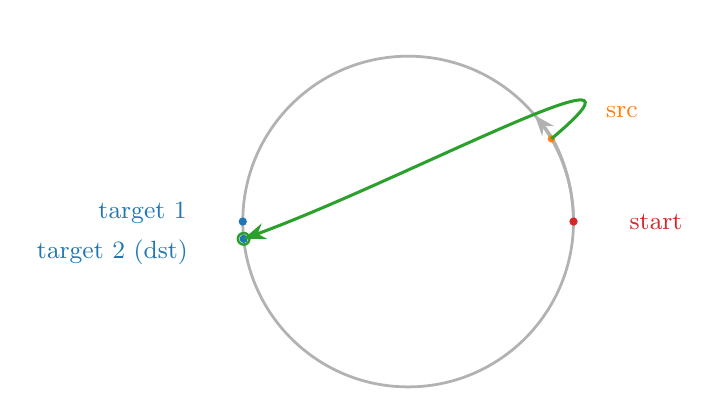
\begin{tikzpicture}[scale=2.1, >=Stealth]
    \def\N{60}
    \def\start{0}
    \def\tone{30}
    \def\ttwo{31}
    \def\src{5}
    \def\R{1.0}
    \coordinate (C) at (0,0);
    \pgfmathsetmacro{\angStart}{360*\start/\N}
    \pgfmathsetmacro{\angTone}{360*\tone/\N}
    \pgfmathsetmacro{\angTtwo}{360*\ttwo/\N}
    \pgfmathsetmacro{\angSrc}{360*\src/\N}
    \coordinate (S) at ({\R*cos(\angStart)},{\R*sin(\angStart)});
    \coordinate (T1) at ({\R*cos(\angTone)},{\R*sin(\angTone)});
    \coordinate (T2) at ({\R*cos(\angTtwo)},{\R*sin(\angTtwo)});
    \coordinate (U) at ({\R*cos(\angSrc)},{\R*sin(\angSrc)});

    \draw[gray!60,line width=1.0pt] (C) circle (\R);
    \draw[->,gray!60,line width=1.0pt] (\R,0) arc (0:40:\R);

    \fill[accentE] (S) circle (0.025);
    \fill[accentA] (T1) circle (0.025);
    \fill[accentA] (T2) circle (0.025);
    \draw[accentC,line width=0.9pt] (T2) circle (0.035);
    \fill[accentB] (U) circle (0.022);

    \node[anchor=west, font=\small, text=accentE] at ($(C)!1.28!(S)$) {start};
    \node[anchor=east, font=\small, text=accentA] at ($(C)!1.28!(T1)+(0,0.05)$) {target 1};
    \node[anchor=east, font=\small, text=accentA] at ($(C)!1.28!(T2)+(0,-0.05)$) {target 2 (dst)};
    \node[anchor=west, font=\small, text=accentB] at ($(C)!1.28!(U)+(0.03,0.02)$) {src};

    \draw[->,accentC,line width=1.1pt] (U) to[out=40,in=20,looseness=1.35] (T2);
  \end{tikzpicture}
  \caption{Geometry for the two-target lazy ring with a directed shortcut (parameters of the shortcut cases).}
  \label{fig:geometry}
\end{figure}

\paragraph{Explicit configurations (all indices modulo $N$).}
Start node is always $n_0=0$. The two targets and shortcut settings for the representative cases are:
\begin{itemize}
  \item \textbf{Case A (no shortcut, $K=2$):} $N=20$, targets $(m_1,m_2)=(18,10)$, $q=2/3$, $g=0.6$, $\beta=0$.
  \item \textbf{Case B (no shortcut, $K=4$):} $N=30$, targets $(m_1,m_2)=(27,15)$, $q=2/3$, $g=0.6$, $\beta=0$.
  \item \textbf{Cases C/D (shortcut, $K=2/4$):} $N=60$, targets $(m_1,m_2)=(30,31)$, $\mathrm{src}=5$, $\mathrm{dst}=31$,
  $q=2/3$, $g=0$, $\beta=0.02$.
  \item \textbf{Case E (three-peak, no shortcut, $K=4$):} $N=30$, targets $(m_1,m_2)=(29,20)$, $q=0.9$, $g=0.8$, $\beta=0$.
\end{itemize}
The same configurations are tabulated in Table~\ref{tab:configs}.

\section*{Representative cases: geometry + FPT}
\begin{figure}[!htbp]
  \centering
  \begin{minipage}{0.24\linewidth}
    \centering
    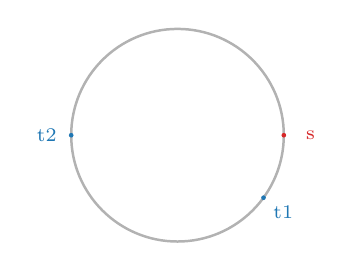
\begin{tikzpicture}[scale=1.35]
      \ringcaseNoSc{20}{0}{18}{10}
    \end{tikzpicture}
  \end{minipage}%
  \hfill
  \begin{minipage}{0.72\linewidth}
    \centering
    \begin{tikzpicture}
      \begin{axis}[
        fptaxislin,
        xmin=0, xmax=60,
        ymin=0, ymax=0.06,
        title={Case A: no shortcut ($K=2$, $g=0.6$)},
      ]
        \addplot[accentA, very thick] table [x=t, y=f_total, col sep=comma] {outputs/A_no_sc_K2_fpt.csv};
        \addplot[black!35, dashed] coordinates {(2,0) (2,0.06)};
        \addplot[black!35, dashed] coordinates {(20,0) (20,0.06)};
        \addplot[only marks, mark=*, mark size=1.6, accentB]
          coordinates {(2,0.0177778) (20,0.0529520)};
        \node[font=\scriptsize, fill=white, fill opacity=0.85, text opacity=1, inner sep=1pt, xshift=6pt, yshift=8pt]
          at (axis cs:2,0.0177778) {$t_1=2$};
        \node[font=\scriptsize, fill=white, fill opacity=0.85, text opacity=1, inner sep=1pt, xshift=-6pt, yshift=8pt]
          at (axis cs:20,0.0529520) {$t_2=20$};
      \end{axis}
    \end{tikzpicture}
  \end{minipage}
  \caption{Case A: geometry and bimodal FPT (peaks marked by dots; dashed lines at $t_1,t_2$).}
  \label{fig:caseA}
\end{figure}

\begin{figure}[!htbp]
  \centering
  \begin{minipage}{0.24\linewidth}
    \centering
    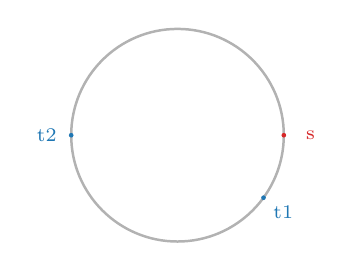
\begin{tikzpicture}[scale=1.35]
      \ringcaseNoSc{30}{0}{27}{15}
    \end{tikzpicture}
  \end{minipage}%
  \hfill
  \begin{minipage}{0.72\linewidth}
    \centering
    \begin{tikzpicture}
      \begin{axis}[
        fptaxislin,
        xmin=0, xmax=60,
        ymin=0, ymax=0.045,
        title={Case B: no shortcut ($K=4$, $g=0.6$)},
      ]
        \addplot[accentA, very thick] table [x=t, y=f_total, col sep=comma] {outputs/B_no_sc_K4_fpt.csv};
        \addplot[black!35, dashed] coordinates {(3,0) (3,0.045)};
        \addplot[black!35, dashed] coordinates {(20,0) (20,0.045)};
        \addplot[only marks, mark=*, mark size=1.6, accentB]
          coordinates {(3,0.0097778) (20,0.0373013)};
        \node[font=\scriptsize, fill=white, fill opacity=0.85, text opacity=1, inner sep=1pt, xshift=6pt, yshift=8pt]
          at (axis cs:3,0.0097778) {$t_1=3$};
        \node[font=\scriptsize, fill=white, fill opacity=0.85, text opacity=1, inner sep=1pt, xshift=-6pt, yshift=8pt]
          at (axis cs:20,0.0373013) {$t_2=20$};
      \end{axis}
    \end{tikzpicture}
  \end{minipage}
  \caption{Case B: geometry and bimodal FPT (peaks marked by dots; dashed lines at $t_1,t_2$).}
  \label{fig:caseB}
\end{figure}

\begin{figure}[!htbp]
  \centering
  \begin{minipage}{0.24\linewidth}
    \centering
    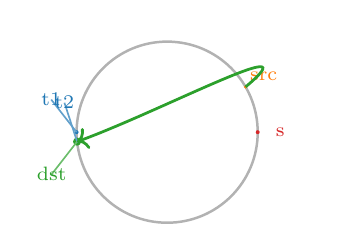
\begin{tikzpicture}[scale=1.15]
      \ringcaseScOverlap{60}{0}{30}{31}{5}{31}
    \end{tikzpicture}
  \end{minipage}%
  \hfill
  \begin{minipage}{0.72\linewidth}
    \centering
    \begin{tikzpicture}
      \begin{axis}[
        fptaxislin,
        xmin=0, xmax=500,
        ymin=0, ymax=0.0010,
        title={Case C: shortcut ($K=2$, $\beta=0.02$)},
      ]
        \addplot[accentA, very thick] table [x=t, y=f_total, col sep=comma] {outputs/C_sc_K2_fpt.csv};
        \addplot[black!35, dashed] coordinates {(36,0) (36,0.0010)};
        \addplot[black!35, dashed] coordinates {(387,0) (387,0.0010)};
        \addplot[only marks, mark=*, mark size=1.6, accentB]
          coordinates {(36,0.000313811) (387,0.000801570)};
        \node[font=\scriptsize, fill=white, fill opacity=0.85, text opacity=1, inner sep=1pt, xshift=6pt, yshift=8pt]
          at (axis cs:36,0.000313811) {$t_1=36$};
        \node[font=\scriptsize, fill=white, fill opacity=0.85, text opacity=1, inner sep=1pt, xshift=-6pt, yshift=8pt]
          at (axis cs:387,0.000801570) {$t_2=387$};
      \end{axis}
    \end{tikzpicture}
  \end{minipage}
  \caption{Case C: geometry and bimodal FPT (peaks marked by dots; dashed lines at $t_1,t_2$).}
  \label{fig:caseC}
\end{figure}

\begin{figure}[!htbp]
  \centering
  \begin{minipage}{0.24\linewidth}
    \centering
    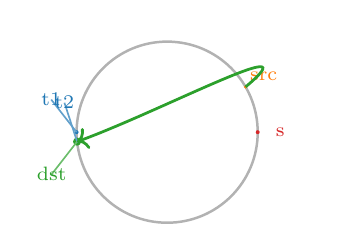
\begin{tikzpicture}[scale=1.15]
      \ringcaseScOverlap{60}{0}{30}{31}{5}{31}
    \end{tikzpicture}
  \end{minipage}%
  \hfill
  \begin{minipage}{0.72\linewidth}
    \centering
    \begin{tikzpicture}
      \begin{axis}[
        fptaxislin,
        xmin=0, xmax=250,
        ymin=0, ymax=0.0022,
        title={Case D: shortcut ($K=4$, $\beta=0.02$)},
      ]
        \addplot[accentA, very thick] table [x=t, y=f_total, col sep=comma] {outputs/D_sc_K4_fpt.csv};
        \addplot[black!35, dashed] coordinates {(15,0) (15,0.0022)};
        \addplot[black!35, dashed] coordinates {(169,0) (169,0.0022)};
        \addplot[only marks, mark=*, mark size=1.6, accentB]
          coordinates {(15,0.000319354) (169,0.00183952)};
        \node[font=\scriptsize, fill=white, fill opacity=0.85, text opacity=1, inner sep=1pt, xshift=6pt, yshift=8pt]
          at (axis cs:15,0.000319354) {$t_1=15$};
        \node[font=\scriptsize, fill=white, fill opacity=0.85, text opacity=1, inner sep=1pt, xshift=-6pt, yshift=8pt]
          at (axis cs:169,0.00183952) {$t_2=169$};
      \end{axis}
    \end{tikzpicture}
  \end{minipage}
  \caption{Case D: geometry and bimodal FPT (peaks marked by dots; dashed lines at $t_1,t_2$).}
  \label{fig:caseD}
\end{figure}

\begin{figure}[!htbp]
  \centering
  \begin{minipage}{0.26\linewidth}
    \centering
    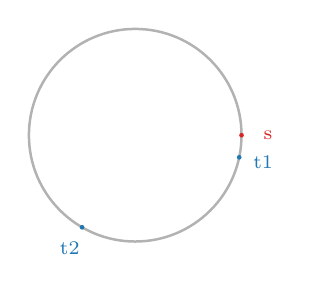
\begin{tikzpicture}[scale=1.35]
      \ringcaseNoSc{30}{0}{29}{20}
    \end{tikzpicture}
  \end{minipage}\hfill
  \begin{minipage}{0.70\linewidth}
    \centering
    \begin{tikzpicture}
      \begin{axis}[
        fptaxislin,
        xmin=0, xmax=90,
        ymin=0, ymax=0.08,
        title={Case E: three peaks ($K=4$, $g=0.8$)},
      ]
        \addplot[accentA, very thick] table [x=t, y=f_total, col sep=comma] {outputs/E_triple_K4_fpt.csv};
        \addplot[black!35, dashed] coordinates {(1,0) (1,0.08)};
        \addplot[black!35, dashed] coordinates {(17,0) (17,0.08)};
        \addplot[black!35, dashed] coordinates {(43,0) (43,0.08)};
        \addplot[only marks, mark=*, mark size=1.6, accentB]
          coordinates {(1,0.045) (17,0.0704637) (43,0.00417010)};
        \node[font=\scriptsize, fill=white, fill opacity=0.85, text opacity=1, inner sep=1pt, xshift=6pt, yshift=8pt]
          at (axis cs:1,0.045) {$t_1=1$};
        \node[font=\scriptsize, fill=white, fill opacity=0.85, text opacity=1, inner sep=1pt, xshift=6pt, yshift=8pt]
          at (axis cs:17,0.0704637) {$t_2=17$};
        \node[font=\scriptsize, fill=white, fill opacity=0.85, text opacity=1, inner sep=1pt, xshift=-6pt, yshift=8pt]
          at (axis cs:43,0.00417010) {$t_3=43$};
      \end{axis}
    \end{tikzpicture}
  \end{minipage}
  \caption{Case E: geometry and three-peak FPT (peaks marked by dots; dashed lines at peak times).}
  \label{fig:caseE}
\end{figure}

\section*{Model and full two-target absorption mechanism}
\paragraph{Lazy ring and drift.}
The ring has $N$ nodes indexed by $0,1,\dots,N-1$. At each step, the walker stays with probability $1-q$ and moves with probability $q$.
For $K=2$ (steps $\pm1$) and $K=4$ (steps $\pm1,\pm2$), a drift parameter $g\in[-1,1]$ splits the move probability:
\begin{align}
  P(+)=\frac{q(1+g)}{2},\qquad P(-)=\frac{q(1-g)}{2},
\end{align}
and the same-direction step lengths share this mass (e.g., for $K=4$, $+1$ and $+2$ each get $P(+)/2$).

\paragraph{Shortcut (selfloop rule).}
Only at the source node $\mathrm{src}$, a fraction of the self-loop is diverted to a shortcut $\mathrm{src}\to\mathrm{dst}$:
\begin{align}
  p=\beta(1-q),\qquad P(\mathrm{src}\to\mathrm{src})=1-q-p,\qquad P(\mathrm{src}\to\mathrm{dst})=p.
\end{align}
All other nodes follow the base ring dynamics.

\paragraph{Exact two-target recursion.}
Let $m_1,m_2$ be absorbing targets. After one step, any mass at the targets is absorbed:
\begin{align}
  \mathbf{p}_{t+1}=\mathbf{p}_t\mathbf{W},\qquad
  f_i(t+1)=[\mathbf{p}_{t+1}]_{m_i},\qquad
  \mathbf{p}_{t+1}(m_i)=0,\ i\in\{1,2\}.
\end{align}
Thus $f(t)=f_1(t)+f_2(t)$, and survival is $S(t)=\sum_i p_t(i)$ with $S(t+1)=S(t)-f(t+1)$.
This gives the exact time-domain FPT distribution without Monte Carlo.

\paragraph{Absorbing Markov chain form (full mechanism).}
Partition the transition matrix as
\begin{align}
\mathbf{W}=\begin{pmatrix}\mathbf{Q} & \mathbf{R}\\ 0 & I\end{pmatrix},
\end{align}
where $\mathbf{Q}$ is the transient subchain and $\mathbf{R}$ contains transitions into the two absorbing states.
Let $\mathbf{r}_i$ be the column of $\mathbf{R}$ for target $m_i$ and $\mathbf{p}_0$ be the initial distribution. Then
\begin{align}
  f_i(t+1)=\mathbf{r}_i^{\mathsf T}\mathbf{Q}^{t}\mathbf{p}_0,\qquad
  f(t+1)=\mathbf{r}^{\mathsf T}\mathbf{Q}^{t}\mathbf{p}_0,
\end{align}
with $\mathbf{r}=\mathbf{r}_1+\mathbf{r}_2$.
In generating-function form,
\begin{align}
  \widetilde f_i(z)=z\,\mathbf{r}_i^{\mathsf T}(I-z\mathbf{Q})^{-1}\mathbf{p}_0.
\end{align}
Equivalently, the survival function is
\begin{align}
  S(t)=\mathbf{1}^{\mathsf T}\mathbf{Q}^{t}\mathbf{p}_0,\qquad f(t+1)=S(t)-S(t+1),
\end{align}
so the two-target FPT is entirely determined by $\mathbf{Q}$ and the two columns $\mathbf{r}_1,\mathbf{r}_2$.
If $\mathbf{Q}$ is diagonalizable, $\mathbf{Q}=\mathbf{V}\mathbf{\Lambda}\mathbf{V}^{-1}$,
then
\begin{align}
  f(t+1)=\sum_k c_k\,\lambda_k^{\,t},
\end{align}
so multiple peaks arise when several modes with distinct time scales (distinct $|\lambda_k|$) carry comparable weights.
This is the complete mathematical mechanism: the time-domain distribution is a weighted sum of $\mathbf{Q}$-powers,
while the frequency-domain response is governed by the resolvent $(I-z\mathbf{Q})^{-1}$.

\paragraph{Connection to Giuggioli's multi-target formula.}
For any graph, the single-target first-passage generating function satisfies
\begin{align}
  \widetilde F_{i\to j}(z)=\frac{\widetilde P_i(j;z)}{\widetilde P_j(j;z)}.
\end{align}
For two targets, the splitting FPT is a $2\times2$ determinant ratio\cite{giuggioli2023}. If
$G_k=\widetilde F_{n_0\to m_k}(z)$ and $F_{jk}$ are built from target-to-target passages and return terms, then
\begin{align}
\widetilde F_{n_0\to (m_1\mid m_2)}(z)=\frac{G_1F_{22}-F_{12}G_2}{F_{11}F_{22}-F_{12}F_{21}},
\end{align}
with the other target obtained by symmetry. The total FPT is the sum of the two splitting distributions.
For partial absorption $\rho_k$, the diagonal terms become
\begin{align}
  F_{kk}=1+\frac{1-\rho_k}{\rho_k}\,[1-R_{m_k}(z)],
\end{align}
where $R_{m_k}(z)$ is the return generating function at target $m_k$ (excluding absorption by the other target).
In my $\rho_1=\rho_2=1$ cases, $F_{11}=F_{22}=1$ and the formula simplifies.

\paragraph{Why multiple peaks appear.}
Multiple peaks arise from multiple path families / time scales.
Drift creates a fast counter-drift family and a slow along-drift family; shortcuts create fast shortcut paths and slow non-shortcut paths.
Two targets further split the probability mass and enhance the visibility of separated modes.

\section*{No shortcut: drift-driven bimodality}
Cases A/B (Figs.~\ref{fig:caseA}--\ref{fig:caseB}) show drift-driven bimodality without shortcuts; Fig.~\ref{fig:splitting} shows splitting contributions.

\begin{figure}[!htbp]
  \centering
  \begin{tikzpicture}
    \begin{semilogyaxis}[
      fptaxis,
      width=0.86\linewidth,
      title={splitting by targets (no shortcut, $K=2$)},
      xmin=0, xmax=140,
      ymin=1e-12, ymax=1,
      legend style={at={(0.02,0.98)}, anchor=north west},
    ]
      \addplot[black!70, thick] table [x=t, y=f_total, col sep=comma] {outputs/A_no_sc_K2_fpt.csv};
      \addplot[accentC, dashed] table [x=t, y=f_target1, col sep=comma] {outputs/A_no_sc_K2_fpt.csv};
      \addplot[accentB, dashed] table [x=t, y=f_target2, col sep=comma] {outputs/A_no_sc_K2_fpt.csv};
      \legend{total,target 1,target 2}
    \end{semilogyaxis}
  \end{tikzpicture}
  \caption{Target splitting: total FPT equals target-1 plus target-2 components.}
  \label{fig:splitting}
\end{figure}

\section*{With shortcut: fast/slow channel superposition}
Cases C/D (Figs.~\ref{fig:caseC}--\ref{fig:caseD}) show shortcut-induced bimodality; Fig.~\ref{fig:scan} shows the $(N,\beta)$ bimodality map (0=no, 1=paper, 2=macro).

\begin{figure}[!htbp]
  \centering
  \begin{minipage}{0.45\linewidth}
    \centering
    \textbf{(a) $K=2$}\par
    \begin{tikzpicture}
      \begin{axis}[
        scanaxis,
        width=0.76\linewidth,
        xlabel={$\beta$}, ylabel={$N$},
        title={bimodality map},
        mesh/cols=9,
      ]
        \addplot[matrix plot*, point meta=explicit]
          table [x=beta, y=N, meta=flag, col sep=comma] {data/scan_bimodality_K2.csv};
      \end{axis}
    \end{tikzpicture}
  \end{minipage}%
  \hfill
  \begin{minipage}{0.45\linewidth}
    \centering
    \textbf{(b) $K=4$}\par
    \begin{tikzpicture}
      \begin{axis}[
        scanaxis,
        width=0.76\linewidth,
        xlabel={$\beta$}, ylabel={$N$},
        title={bimodality map},
        mesh/cols=9,
      ]
        \addplot[matrix plot*, point meta=explicit]
          table [x=beta, y=N, meta=flag, col sep=comma] {data/scan_bimodality_K4.csv};
      \end{axis}
    \end{tikzpicture}
  \end{minipage}
  \caption{Bimodality map (0=no, 1=paper, 2=macro) with $\mathrm{src}=5$, $\mathrm{dst}=m_2$, $m_1=\lfloor N/2\rfloor$, $m_2=m_1+1$.}
  \label{fig:scan}
\end{figure}

\section*{Three-peak example}
Case E (Fig.~\ref{fig:caseE}) shows a three-peak case driven by strong drift and $K=4$ jump-over.

\section*{Configurations and reproducibility}
Tables~\ref{tab:configs} and~\ref{tab:peaks} summarize the representative cases and peak metrics.
Reproduce with:
\begin{verbatim}
cd reports/ring_two_target
python3 code/two_target_report.py
latexmk -pdf -auxdir=build -emulate-aux-dir ring_two_target_en.tex
\end{verbatim}

\begin{table}[!htbp]
  \centering
  \caption{Representative configurations (see \texttt{data/model\_configs.csv}).}
  \label{tab:configs}
  \begin{tabular}{lllllll}
\toprule
Case & $N$ & $K$ & $q$ & $g$ & $\beta$ & targets \\
\midrule
A\_no\_sc\_K2 & 20 & 2 & 0.667 & 0.60 & 0.000 & (18,10) \\
B\_no\_sc\_K4 & 30 & 4 & 0.667 & 0.60 & 0.000 & (27,15) \\
C\_sc\_K2 & 60 & 2 & 0.667 & 0.00 & 0.020 & (30,31) \\
D\_sc\_K4 & 60 & 4 & 0.667 & 0.00 & 0.020 & (30,31) \\
E\_triple\_K4 & 30 & 4 & 0.900 & 0.80 & 0.000 & (29,20) \\
\bottomrule
\end{tabular}
\end{table}

\begin{table}[!htbp]
  \centering
  \caption{Peak locations and criteria ($t_1$ earliest peak, $t_2$ latest peak).}
  \label{tab:peaks}
  \begin{tabular}{llllllll}
\toprule
Case & $t_1$ & $h_1$ & $t_2$ & $h_2$ & $h_2/h_1$ & paper & macro \\
\midrule
A\_no\_sc\_K2 & 2 & 1.78e-02 & 20 & 5.30e-02 & 2.98 & True & True \\
B\_no\_sc\_K4 & 3 & 9.78e-03 & 20 & 3.73e-02 & 3.81 & True & False \\
C\_sc\_K2 & 36 & 3.14e-04 & 387 & 8.02e-04 & 2.55 & True & True \\
D\_sc\_K4 & 15 & 3.19e-04 & 169 & 1.84e-03 & 5.76 & True & True \\
E\_triple\_K4 & 1 & 4.50e-02 & 43 & 4.17e-03 & 0.09 & True & True \\
\bottomrule
\end{tabular}
\end{table}

\begin{thebibliography}{9}
\bibitem{giuggioli2023}
L. Giuggioli et al., \emph{Multi-target search in bounded and heterogeneous environments: a lattice random walk perspective}, arXiv:2311.00464v2.
\bibitem{sarvaharman2020}
A. Sarvaharman and L. Giuggioli, \emph{Phys. Rev. E} 102, 062124 (2020).
\end{thebibliography}

\end{document}
